\usetikzlibrary{arrows.meta}
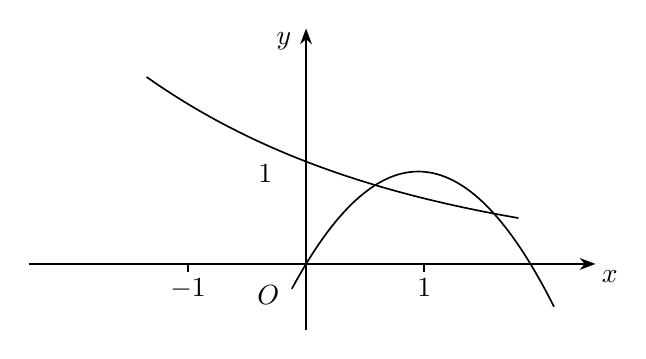
\begin{tikzpicture}[x=1.5cm,y=1.3cm,line width=.6pt,>=Stealth]
\tikzset{
  axis/.style={->},
  tick/.style={},
  curve/.style={},
  guide/.style={dashed},
  xlab/.style={anchor=west,inner sep=0pt},
  ylab/.style={anchor=east,inner sep=0pt},
  olab/.style={anchor=north east,inner sep=0pt},
  tlab/.style={anchor=north,inner sep=0pt},
  yticklab/.style={anchor=east,inner sep=0pt}
}
\coordinate (xmin) at (-2.35,0);
\coordinate (xmax) at (2.45,0);
\coordinate (ymin) at (0,-0.65);
\coordinate (ymax) at (0,2.3);
\coordinate (O) at (0,0);
\coordinate (tm) at (-1,0);
\coordinate (tmb) at (-1,-0.08);
\coordinate (tp) at (1,0);
\coordinate (tpb) at (1,-0.08);
\coordinate (root2) at (1.9,0);
\coordinate (vertex) at (0.95,0.9025);
\coordinate (pleft) at (-0.12,-0.2424);
\coordinate (pright) at (2.1,-0.42);
\coordinate (exp0) at (0,1);
\coordinate (expL) at (-1.35,1.8271);
\coordinate (expR) at (1.8,0.4478);
\coordinate (i1) at (0.586,0.7704);
\coordinate (i2) at (1.591,0.4918);
\draw[axis] (xmin)--(xmax);
\draw[axis] (ymin)--(ymax);
\draw[tick] (tm)--(tmb);
\draw[tick] (tp)--(tpb);
\draw[curve,domain=-0.12:2.1,samples=181] plot (\x,{(\x)*(1.9-(\x))});
\draw[curve,domain=-1.35:1.8,samples=181] plot (\x,{0.64^(\x)});
\node[anchor=north west,inner sep=0pt,xshift=2pt,yshift=-2pt] at (xmax) {$x$};
\node[ylab] at (-0.12,2.18) {$y$};
\node[olab] at (-0.22,-0.2) {$O$};
\node[yticklab] at (-0.28,0.88) {$1$};
\node[tlab] at (-1,-0.14) {$-1$};
\node[tlab] at (1,-0.14) {$1$};
\end{tikzpicture}
